%"The PDF file may contain up to 25 pages of reference material, single-sided, letter or A4 size, with text and illustrations readable by a person with correctable eyesight without magnification from a distance of 1/2 meter."
\documentclass[10pt,landscape,twocolumn,a4paper,notitlepage]{article}
\usepackage{hyperref}
\usepackage[spanish, activeacute]{babel}
\usepackage[utf8]{inputenc}
\usepackage{fancyhdr}
\usepackage{lastpage}
\usepackage{listings}
\usepackage{amssymb}
\usepackage[usenames,dvipsnames]{color}
\usepackage{graphicx}
\usepackage{wrapfig}
\usepackage{amsmath}
\usepackage{makeidx}
\usepackage{ifthen}
\usepackage{xcolor}

%%% Margenes
\setlength{\columnsep}{0.25in}    % default=10pt
\setlength{\columnseprule}{0.5pt}    % default=0pt (no line)

\addtolength{\textheight}{2.75in}
\addtolength{\topmargin}{-1.1in}

\addtolength{\textwidth}{1.7in}
\addtolength{\oddsidemargin}{-0.8in}

\setlength{\headsep}{0.08in}
\setlength{\parskip}{0in}
\setlength{\headheight}{12pt}
\setlength{\parindent}{0mm}

%%% Encabezado y pie de pagina
\pagestyle{fancy}
\fancyhead[LO]{\textbf{\title}}
%\fancyhead[C]{\leftmark\ -\ \rightmark}
\fancyhead[RO]{Página \thepage\ of \pageref{LastPage}}
\renewcommand{\headrulewidth}{0.4pt}
\fancyfoot{}
\definecolor{darkblue}{rgb}{0,0,0.4}
%%% Configuracion de Listings
\lstloadlanguages{C++}
\lstnewenvironment{code}
	{%\lstset{	numbers=none, frame=lines, basicstyle=\small\ttfamily, }%
	 \csname lst@SetFirstLabel\endcsname}
	{\csname lst@SaveFirstLabel\endcsname}
\lstset{% general command to set parameter(s)
	language=C++, basicstyle=\small\ttfamily, keywordstyle=\slshape,
	emph=[1]{tipo,usa}, emphstyle={[1]\sffamily\bfseries},
	morekeywords={tint,forn,forsn,fore},
	basewidth={0.47em,0.40em},
	columns=fixed, fontadjust, resetmargins, xrightmargin=5pt, xleftmargin=15pt,
	flexiblecolumns=false, tabsize=2, breaklines,	breakatwhitespace=false, extendedchars=true,
	numbers=left, numberstyle=\tiny, stepnumber=1, numbersep=9pt,
	frame=l, framesep=3pt,
    basicstyle=\ttfamily,
    keywordstyle=\color{darkblue}\ttfamily,
    stringstyle=\color{magenta}\ttfamily,
    commentstyle=\color{RedOrange}\ttfamily,
    morecomment=[l][\color{OliveGreen}]{\#}
}

\lstdefinestyle{C++}{
	language=C++, basicstyle=\small\ttfamily, keywordstyle=\slshape,
	emph=[1]{tipo,usa,tipo2}, emphstyle={[1]\sffamily\bfseries},
	morekeywords={tint,forn,forsn,fore},
	basewidth={0.47em,0.40em},
	columns=fixed, fontadjust, resetmargins, xrightmargin=5pt, xleftmargin=15pt,
	flexiblecolumns=false, tabsize=2, breaklines,	breakatwhitespace=false, extendedchars=true,
	numbers=left, numberstyle=\tiny, stepnumber=1, numbersep=9pt,
	frame=l, framesep=3pt,
    basicstyle=\ttfamily,
    keywordstyle=\color{darkblue}\ttfamily,
    stringstyle=\color{magenta}\ttfamily,
    commentstyle=\color{RedOrange}\ttfamily,
    morecomment=[l][\color{OliveGreen}]{\#}
}

%%% Macros
\def\nbtitle#1{\begin{Large}\begin{center}\textbf{#1}\end{center}\end{Large}}
\def\nbsection#1{\section{#1}}
\def\nbsubsection#1{\subsection{#1}}
\def\nbcoment#1{\begin{small}\textbf{#1}\end{small}}
\newcommand{\comb}[2]{\left( \begin{array}{c} #1 \\ #2 \end{array}\right)}
\def\complexity#1{\texorpdfstring{$\mathcal{O}(#1)$}{O(#1)}}


% command cppfile(linerange, file)
% Muestra las lineas dadas por 'linerange' en el archivo 'file'
%
% Ejemplos:
%
% \cppfile{9-10,15,20-22}{template.cpp}
% muestra las lineas 9,10,15,20,21,22 de 'template.cpp'
%
% \cppfile{}{segtree.cpp}
% muestra todas las lineas de 'segtree.cpp'
\newcommand{\cppfile}[2]{ \lstinputlisting[style=C++,linerange={#1}]{#2} }

\newcommand{\yesno}[2]{
	\ifthenelse{\equal{#1}{y}}{\textcolor{teal}{#2}}{\textcolor{red}{#2}}
}

\newcommand{\usedby}[3]{
	\textbf{[\yesno{#1}{KR}\yesno{#2}{MX}\yesno{#3}{SR}]}
}

\begin{document}

\def\title{Instituto Tecnológico de Costa Rica campus Alajuela - Todo Es mental}
\textcolor{white}{.}\\[0.2cm]
\centering{\LARGE\textbf{Todo Es mental}} \\[0.5cm]
\centering{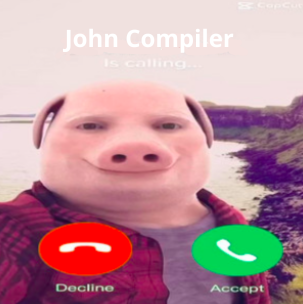
\includegraphics[width=5.5cm]{img/logo.png}}
\tableofcontents\newpage

\section{Fuentes}
	\begin{itemize}
		\item \url{https://github.com/kth-competitive-programming/kactl}
		\item \url{https://github.com/brunomaletta/Biblioteca}
		\item \url{https://github.com/francoderico/la-pandilla}
		\item \url{https://github.com/mhunicken/icpc-team-notebook-el-vasito}
		\item \url{https://github.com/vmartinv/eldiego}
		\item \url{https://cp-algorithms.com}
	\end{itemize}

% Red para cada quién que no lo haya utilizado
% Green para cada quién que sí lo haya utilizado
% \textcolor{red}{M}\textcolor{red}{S}\textcolor{red}{K}

\section{Init}
	\subsection{Template}
		\cppfile{}{src/init/init.cpp}
	\subsection{Compilación}
		\cppfile{}{src/init/compile.cpp}
	\subsection{Pragmas}
		\cppfile{}{src/init/pragmas.cpp}
	\subsection{RNG}
		\cppfile{}{src/init/rng.cpp}
	%\subsection{Bit Tricks}

\section{Estructuras}
	\subsection{Fenwick}
		\usedby{n}{y}{n}
		\cppfile{}{src/estructuras/fenwick.cpp}
	\subsection{Fenwick 2D}
		\usedby{n}{n}{n}
		\cppfile{}{src/estructuras/fenwick2d.cpp}
	\subsection{Segment Tree}
		\usedby{n}{y}{n}
		\cppfile{}{src/estructuras/segtree.cpp}
	\subsection{Segment Tree Lazy}
		\usedby{n}{n}{n}
		\cppfile{}{src/estructuras/segtree-lazy.cpp}
	\subsection{Union Find}
		\usedby{n}{y}{n}
		\cppfile{}{src/estructuras/dsu.cpp}
	\subsection{Ordered Set}
		\usedby{n}{y}{n}
		\cppfile{}{src/estructuras/ordered-set.cpp}
	\subsection{Sparse Table}
		\usedby{n}{y}{n}
		\cppfile{}{src/estructuras/sparse-table.cpp}
	\subsection{Fast Unordered Map}
		\usedby{n}{n}{n}
		\cppfile{}{src/estructuras/fast-map.cpp}


\section{Misc}
	\subsection{Matrix Template}
		\usedby{n}{n}{n}
		\cppfile{}{src/misc/matrix.cpp}
	\subsection{Mod Template}
		\usedby{n}{n}{n}
		\cppfile{}{src/misc/mod.cpp}
	\subsection{Mo's}
		\usedby{n}{y}{n}
		\cppfile{}{src/misc/mos.cpp}

\section{Flujos y Matchings}
	\subsection{Push Relabel}
		\usedby{n}{n}{n}
		\cppfile{}{src/flujos_matching/push_relabel.cpp}
	\subsection{Hopcroft Karp}
		\usedby{n}{n}{n}
		\cppfile{}{src/flujos_matching/hopcroft_karp.cpp}
	\subsection{Min Cost Max Flow}
		\usedby{n}{n}{n}
		\cppfile{}{src/flujos_matching/min_cost_max_flow.cpp}
	\subsection{Hungarian}
		\usedby{n}{n}{n}
		\cppfile{}{src/flujos_matching/hungarian.cpp}
	\subsection{Dinitz's}
		\usedby{n}{y}{n}
		\cppfile{}{src/flujos_matching/dinitz.cpp}
	\subsection{Flow with requirements}
		\usedby{n}{n}{n}
		\cppfile{}{src/flujos_matching/lowerboundflow.cpp}

\section{Grafos}
	\subsection{Toposort}
		\usedby{n}{y}{n}
		\cppfile{}{src/grafos/topo_sort.cpp}
	\subsection{SCC}
		\usedby{n}{y}{n}
		\cppfile{}{src/grafos/scc-tarjan.cpp}
	\subsection{Dijkstra and BFS 0-1}
		\usedby{n}{y}{n}
		\cppfile{}{src/grafos/dijkstra.cpp}
	\subsection{2Sat}
		\usedby{n}{y}{n}
		\cppfile{}{src/grafos/2sat.cpp}
	\subsection{Bellman Ford}
		\usedby{n}{n}{n}
		\cppfile{}{src/grafos/bellman_ford.cpp}
	\subsection{Floyd Washall}
		\usedby{n}{y}{n}
		\cppfile{}{src/grafos/floyd_warshall.cpp}
	\subsection{Euler Path/Cycle}
		\usedby{n}{n}{n}
		\cppfile{}{src/grafos/euler_path_cycle.cpp}
	\subsection{Puntes y Puntos de Articulación}
		\usedby{n}{n}{n}
		\cppfile{}{src/grafos/articulation_points_bridges.cpp }
	\subsection{Kruskal}
		\usedby{n}{y}{n}
		\cppfile{}{src/grafos/kruskal.cpp}
	%\subsection{Blossom}
		%\usedby{n}{n}{n}
	%\subsection{Max Clique and Max Independent Set}
		%\usedby{n}{n}{n}

\section{Árboles}
	\subsection{Binary Lifting for LCA and Kth Ancestor}
		\usedby{n}{y}{n}
		\cppfile{}{src/arboles/lca.cpp}
	\subsection{Centroid Decomposition}
		\usedby{n}{y}{n}
		\cppfile{}{src/arboles/centroid.cpp}
	\subsection{Heavy Light Decomposition}
		\usedby{n}{n}{n}
		\cppfile{}{src/arboles/hld.cpp}
	\subsection{Centro y Diámetro de un Árbol}
		\usedby{n}{n}{n}
		\cppfile{}{src/arboles/center.cpp}

\section{Identidades}
\section{Identidades}
\subsection{Cantidad de primos menores que $10^n$}\ \\
% El diego
$\pi(10^1)$ = 4 ;
$\pi(10^2)$ = 25 ;
$\pi(10^3)$ = 168 ;
$\pi(10^4)$ = 1229 ;
$\pi(10^5)$ = 9592 \\
$\pi(10^6)$ = 78.498 ;
$\pi(10^7)$ = 664.579 ;
$\pi(10^8)$ = 5.761.455 ;
$\pi(10^9)$ = 50.847.534 \\
$\pi(10^{10})$ = 455.052,511 ;
$\pi(10^{11})$ = 4.118.054.813 ;
$\pi(10^{12})$ = 37.607.912.018% ;

\subsection{Divisores} \ \\
Cantidad de divisores ($\sigma_0$) para \emph{algunos} $n / \neg\exists n'<n, \sigma_0(n') \geqslant \sigma_0(n)$ \\
$\sigma_0(60)$ = 12 ; $\sigma_0(120)$ = 16 ; $\sigma_0(180)$ = 18 ; $\sigma_0(240)$ = 20 ; $\sigma_0(360)$ = 24 \\
$\sigma_0(720)$ = 30 ; $\sigma_0(840)$ = 32 ; $\sigma_0(1260)$ = 36 ; $\sigma_0(1680)$ = 40 ; $\sigma_0(10080)$ = 72 \\ $\sigma_0(15120)$ = 80 ; $\sigma_0(50400)$ = 108 ; $\sigma_0(83160)$ = 128 ; $\sigma_0(110880)$ = 144 \\
$\sigma_0(498960)$ = 200 ; $\sigma_0(554400)$ = 216 ; $\sigma_0(1081080)$ = 256 ; $\sigma_0(1441440)$ = 288  $\sigma_0(4324320)$ = 384 ; $\sigma_0(8648640)$ = 448


\subsection{Series}
Fuente: Kactl theorical \\

$$\sum_{i=1}^{n} i^{2} = \frac{n(n+1)(2n+1)}{6}  \qquad  \sum_{i=1}^{n} i^{3} = \frac{n^{2}(n+1)^{2}}{4} = \left(\sum_{i=1}^n i\right)^2$$

$$ g_k(n) = \sum_{i=1}^n i^k = \frac{1}{k+1} \left( n^{k+1} + \sum_{j=1}^k \binom{k+1}{j+1} (-1)^{j+1} g_{k-j}(n) \right) $$

$$\sum_{i=0}^{n} ic^{i} = \frac{nc^{n+2} - (n+1)c^{n+1} + c}{(c-1)^{2}}, \quad c \neq 1$$

$$\sum_{i=0}^{\infty} ic^{i} = \frac{c}{(1-c)^{2}}, \quad |c| < 1$$

\subsection{Identidades binomiales}
Fuente: Kactl theorical \\

\bigskip

$$
\begin{array}{cc}
\binom{n}{k} = \frac{n}{k}\binom{n-1}{k-1}
&
\binom{n-1}{k} - \binom{n-1}{k-1} = \frac{n - 2k}{k} \binom{n}{k}
\\[10pt]
\binom{n}{h}\binom{n-h}{k} = \binom{n}{k}\binom{n-k}{h} &
\binom{n}{k} = \frac{n+1-k}{k} \binom{n}{k-1}
\\[10pt]
\sum_{k = 0}^n k\binom{n}{k} = n 2^{n-1} &
\sum_{k = 0}^n k^2 \binom{n}{k} = (n + n^2)2^{n-2}
\\[10pt]
\sum_{j = 0}^k\binom{m}{j} \binom{n-m}{k-j} = \binom{n}{k} &
\sum_{j = 0}^m \binom{m}{j}^2 = \binom{2m}{m}
\\[10pt]
\sum_{m = 0}^n \binom{m}{j} \binom{n-m}{k-j} = \binom{n+1}{k+1} &
\sum_{m = k}^n \binom{m}{k} = \binom{n+1}{k+1}
\\[10pt]
\sum_{r = 0}^m \binom{n+r}{r} = \binom{n+m+1}{m} &
\sum_{k=0}^{\lfloor n/2 \rfloor} \binom{n-k}{k} = \text{Fib}(n+1)
\\[10pt]
(x + y)^{n} = \sum_{k=0}^{n} \binom{n}{k} x^{n-k} y^{k} &
(1 + x)^{n} = \sum_{k=0}^{n} \binom{n}{k} x^{k}
\\[10pt]
2\sum_{i = L}^R \binom{n}{i} - \binom{n}{L} - \binom{n}{R} = \sum_{i = L+1}^R \binom{n+1}{i}
\end{array}
$$

\subsection{Identidades teoría de números}
Fuente: Kactl theorical \\

$$ \sum_{d|n} \varphi(d) = n$$

$$ \sum_{\substack{i < n \\ \text{gcd}(i, n) = 1}} i = n \cdot \frac{\varphi(n)}{2} $$

$$ |\{(x, y) : \, 1 \leq x, y \leq n, \, \text{gcd}(x, y) = 1\}| = \sum_{d = 1}^n \mu(d) \left \lfloor \frac{n}{d} \right \rfloor^2$$

$$\sum_{x = 1}^n \sum_{y = 1}^n \text{gcd}(x, y)
= \sum_{k = 1}^n k \sum_{k|l}^{n} \left \lfloor \frac{n}{l} \right \rfloor^2 \mu\left(\frac{l}{k}\right)$$

$$\sum_{x = 1}^n \sum_{y = x}^n \text{gcd}(x, y) = \sum_{g = 1}^n \sum_{g|d}^n g \cdot \varphi\left(\frac{d}{g}\right)$$

$$\sum_{x = 1}^n \sum_{y = 1}^n \text{lcm}(x, y)
= \sum_{d = 1}^n d \, \mu(d) \sum_{d|l}^{n} l \binom{\lfloor \frac{n}{l} \rfloor + 1}{2}^2$$

$$\sum_{x = 1}^n \sum_{y = x+1}^n \text{lcm}(x, y) = \sum_{g = 1}^n \sum_{g|d}^n d \cdot \varphi\left(\frac{d}{g}\right) \cdot \frac{d}{g} \cdot \frac 1 2$$

$$\sum_{x \in A} \sum_{y \in A} \text{gcd}(x, y)
= \sum_{t = 1}^n \left(\sum_{l | t} \frac{t}{l} \mu(l)\right) \left(\sum_{t|a} \text{freq}[a]\right)^2$$

$$\sum_{x \in A} \sum_{y \in A} \text{lcm}(x, y)
= \sum_{t = 1}^n \left(\sum_{l | t} \frac{l}{t} \mu(l)\right) \left(\sum_{a \in A, \, t|a} a\right)^2$$

\subsection{Large Prime Gaps}
For numbers until $10^9$ the largest gap is 400.\\
For numbers until $10^{18}$ the largest gap is 1500.\\[0.5cm]

\subsection{Prime counting function - \texorpdfstring{$\pi(x)$}{}} The prime counting function is asymptotic to $\frac{x}{\log x}$, by the prime number theorem.

\ 

\subsection{Some Primes}

999999937 $\quad$ 1000000007 $\quad$ 1000000009 $\quad$ 1000000021 $\quad$ 1000000033
$10^{18} - 11 \quad\quad 10^{18} + 3 \quad\quad\quad 2305843009213693951 = 2^{61} - 1$


\section{Matemática}
	\subsection{GCD Extendido}
		\usedby{n}{n}{n}
		\cppfile{}{src/matematica/gcd_extendido.cpp}
	\subsection{Euler Totient}
		\usedby{n}{n}{n}
		\cppfile{}{src/matematica/totient.cpp}
	\subsection{Criba de Totient}
		\usedby{n}{n}{n}
		\cppfile{}{src/matematica/criba_variaciones.cpp}
	\subsection{Miller-Rabin}
		\usedby{n}{n}{n}
		\cppfile{}{src/matematica/miller_rabin.cpp}
	\subsection{Logaritmo Discreto}
		\usedby{n}{n}{n}
		\cppfile{}{src/matematica/logaritmo_discreto.cpp}
	\subsection{Eliminación Gaussiana}
		\usedby{n}{n}{n}
		\cppfile{}{src/matematica/gauss_elim.cpp}
	\subsection{Determinante}
		\usedby{n}{n}{n}
		\cppfile{}{src/matematica/determinante.cpp}

\section{Geometría 2D}
	\subsection{Point Template}
		\usedby{n}{y}{n}
		\cppfile{}{src/geometria/Point.h}
	\subsection{Convex Hull}
		\usedby{n}{n}{n}
		\cppfile{}{src/geometria/convex_hull.cpp}
	\subsection{Par de puntos más cercanos}
		\usedby{n}{n}{n}
		\cppfile{}{src/geometria/closest_pair.cpp}
	\subsection{Geometria distancias, intersecciones, entre otros}
		\usedby{n}{n}{n}
		\cppfile{}{src/geometria/geo.cpp}
% Meter todo lo demás
% TODO

\section{Transformadas y Convoluciones}
	\subsection{FFT}
		\usedby{n}{y}{n}
		\cppfile{}{src/conv/fft.cpp}
	\subsection{NTT}
		\usedby{n}{n}{n}
		\cppfile{}{src/conv/ntt.cpp}
	\subsection{FWHT}
		\usedby{n}{y}{n}
		\cppfile{}{src/conv/fwht.cpp}
	\subsection{Convoluciones GCD y LCM}
		\usedby{n}{y}{n}
		\cppfile{}{src/conv/gcdlcm.cpp}

\section{Optimización}
	\subsection{Simulated Annealing}
		\usedby{n}{n}{n}
		\cppfile{}{src/heuristica/simulated_annealing.cpp}

%\section{Estructuras}
%\subsection{TEST}
%\cppfile{}{test.cpp}

\end{document}

